\documentclass[12pt,a4paper]{article}
\usepackage[utf8]{vietnam}
\usepackage[utf8]{inputenc}
\usepackage[T1]{fontenc}
\usepackage{fourier}
\usepackage[T5]{fontenc}
\usepackage{amsmath}
\usepackage{amssymb}
\usepackage{graphicx}
\begin{document}
	\section*{Nghiên cứu dự báo giá chứng khoán Tesla}
	
	\subsection{Giới thiệu bài toán, dữ liệu, mô hình}
	Bài toán dự báo giá chứng khoán là một bài toán quan trọng trong lĩnh vực tài chính và kinh doanh. Mục tiêu của bài toán này là dự báo giá chứng khoán trong tương lai dựa trên dữ liệu lịch sử.
	
	Dữ liệu sử dụng cho bài toán này là dữ liệu giá chứng khoán của công ty Tesla (TSLA), bao gồm các thông tin như giá mở cửa, giá đóng cửa, giá cao nhất, giá thấp nhất và số lượng chứng khoán giao dịch. Dữ liệu được thu thập từ trang web \textit{Kaggle.com} và đã được xử lý để loại bỏ các giá trị thiếu và ngoại lệ.
	
	Trong bài báo cáo này, chúng tôi sử dụng các mô hình học máy để dự báo giá chứng khoán TSLA trong tương lai. Đặc biệt, chúng tôi sử dụng mô hình Linear Regression, Decision Tree Regressor và Random Forest Regressor để dự báo và đánh giá chúng \\
	
	\subsection{Giải quyết}
	Để giải quyết bài toán, chúng tôi tiến hành các bước sau:
	
	\begin{enumerate}
		\item Đọc và xử lý dữ liệu \\
		
		Tải dữ liệu giá chứng khoán của TSLA vào một pandas DataFrame và chuyển đổi cột "Date" sang dạng datetime, điều này sẽ giúp cho việc xử lý và đánh giá dữ liệu dễ dàng hơn. Tiến hành xử lý các giá trị thiếu và ngoại lệ bằng cách loại bỏ chúng.
		
		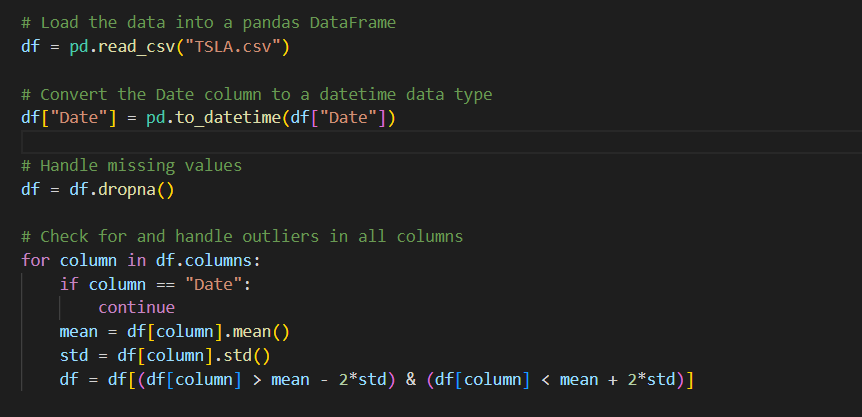
\includegraphics{1}
		
		\item Chuẩn hóa dữ liệu \\ 
		
		Chuẩn hóa tất cả các cột trong DataFrame bằng cách trừ giá trị nhỏ nhất của cột đó và chia cho khoảng giá trị giữa giá trị lớn nhất và nhỏ nhất của cột đó.
		
		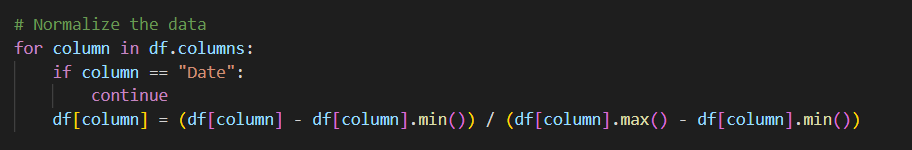
\includegraphics{2}
		
		\item Tách dữ liệu \\ 
		
		Tách dữ liệu thành tập huấn luyện và tập kiểm tra bằng cách chia dữ liệu thành 80\% tập huấn luyện và 20\% tập kiểm tra. \\
		
		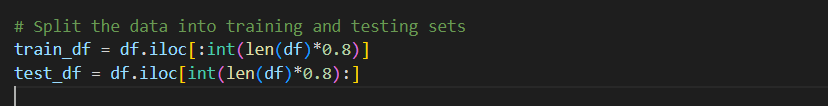
\includegraphics{3}
		
		Sau khi tách dữ liệu được dùng để tính toán và hiển thị ma trận tương quan giữa các cột trong DataFrame. 
		
		Hàm corr() được sử dụng để tính toán các chỉ số tương quan giữa các cột, và hàm sns.heatmap() được sử dụng để tạo ra một heatmap để hiển thị chỉ số tương quan giữa các cột. 
		
		Cụ thể hơn, hàm corr() được gọi trên DataFrame đã chuẩn hóa và tách dữ liệu, để tính toán chỉ số tương quan giữa tất cả các cột trong DataFrame, chú ý tham số numeric\_only=False để tính chỉ số tương quan giữa cả dữ liệu số và chuỗi.
		
		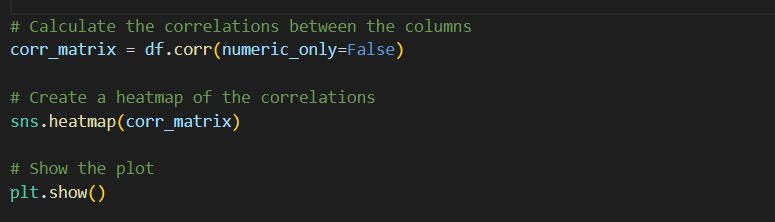
\includegraphics{4}
		
		Sử dụng hàm sns.heatmap để hiển thị chúng trong dạng một heatmap. Heatmap này sẽ cho ta một cái nhìn tổng quát về mối quan hệ giữa các cột trong DataFrame. 
		
		Các màu sắc từ xanh lá đến đỏ sẽ biểu thị mức độ tương quan từ thấp đến cao giữa các cột. 
		
		Chúng ta có thể dùng heatmap này để tìm ra các cột có mối quan hệ cao với nhau, hoặc cột có mối quan hệ thấp với các cột khác.
		
		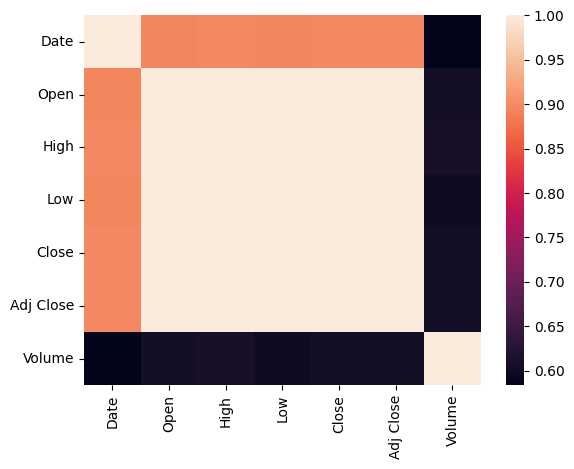
\includegraphics{output1}
		
		\item Đào tạo và đánh giá mô hình
		
		Sử dụng các mô hình Linear Regression, Decision Tree Regressor và Random Forest Regressor để huấn luyện với tập huấn luyện và đánh giá với tập kiểm tra. 
		
		Chúng tôi sử dụng chỉ số mean squared error và root mean squared error để đánh giá chất lượng của các mô hình.
		
		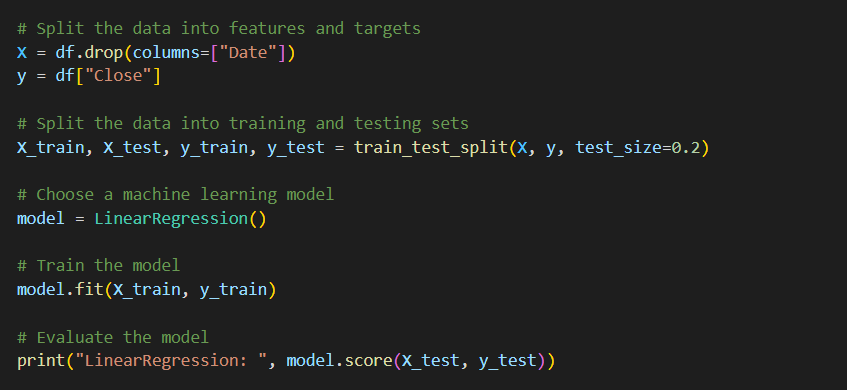
\includegraphics{5}
		
		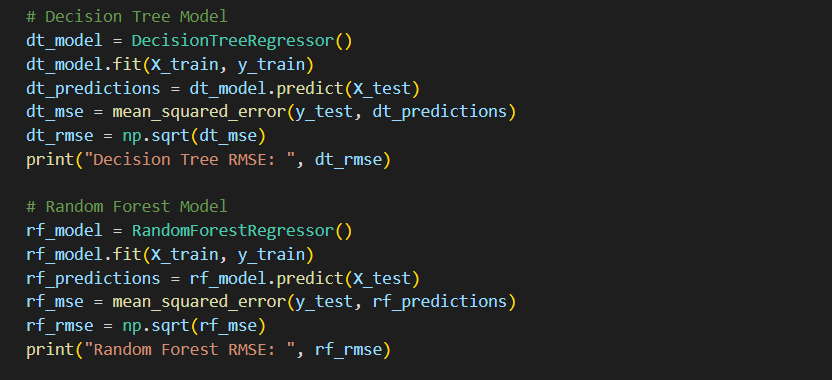
\includegraphics{6}
		
		Đây là kết quả sau khi tiến hành đánh giá các mô hình:
		
		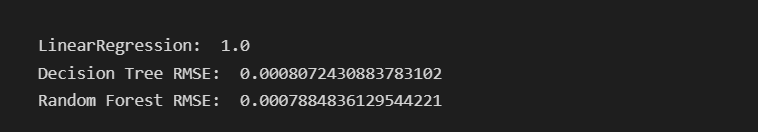
\includegraphics{7}
		
		Vậy, ta chọn mô hình LinearRegression để giải quyết bài toán của chúng ta.
		
		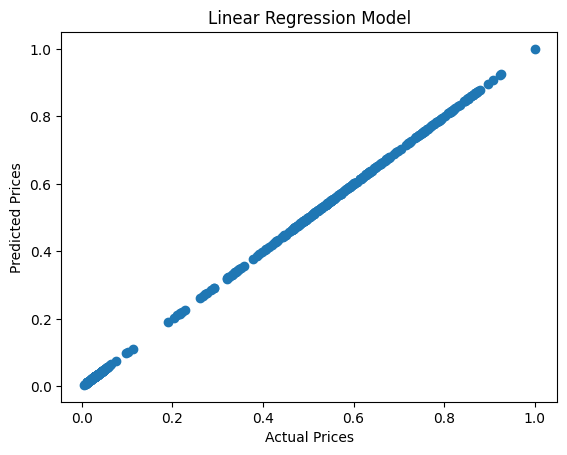
\includegraphics{output2}
		
	\end{enumerate}
	
	\subsection{Ứng dụng trong thực tế}
	\begin{enumerate}
		
		Kết quả của bài báo cáo này có thể được sử dụng để dự báo giá chứng khoán trong tương lai và đưa ra các quyết định đầu tư hợp lý.
		
		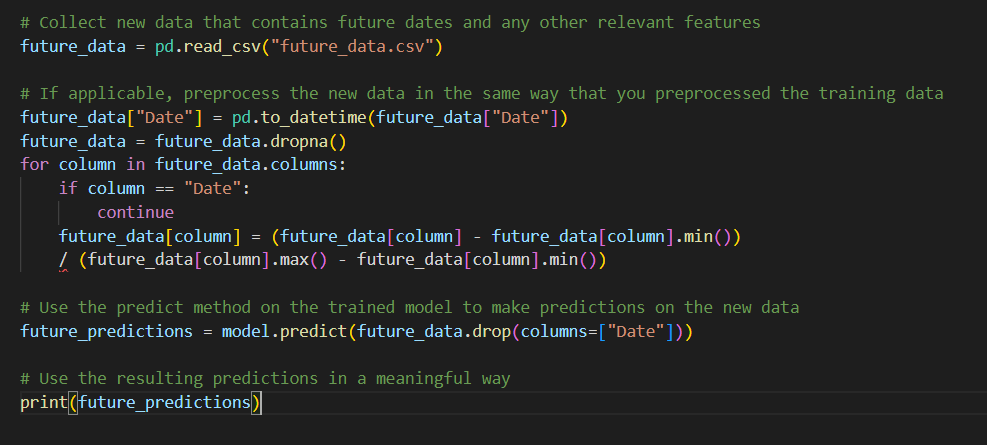
\includegraphics{8}
		
		Tuy nhiên, hiện tại chưa tìm được dữ liệu Stock Tesla 2020-present, nên đoạn code trên chỉ là demo sau khi chúng ta có được dữ liệu tương ứng. 
		
		Các mô hình học máy có thể được sử dụng để dự báo giá chứng khoán của các công ty khác và cả trong các lĩnh vực khác nhau. 
		
		Ngoài ra, kết quả của bài báo cáo này cũng có thể được sử dụng để cải thiện và tinh chỉnh các mô hình học máy cho các bài toán tương tự.
		
	\end{enumerate}
\end{document}